%\newpage
\vspace{-3.5pt}
\section{Problem Definition}
\label{sec:problem-definition}
%\guy{Can someone check Sections 3-4-5? Especially the formulations}


\subsection{Background}
\label{subsec:background}

\textbf{Petri nets.}
A Petri net $N=(P,T,\mathsf{pre},\mathsf{post},M_0)$ has places $P$, transitions $T$, incidence maps $\mathsf{pre},\mathsf{post}:T\to\mathbb N^P$, and initial marking $M_0$.
A transition $t$ is enabled at $M$ if $M\ge \mathsf{pre}(t)$; firing yields $M' = M - \mathsf{pre}(t) + \mathsf{post}(t)$, written $M\xrightarrow{t}M'$.
For a sequence $\sigma$, write $M\xrightarrow{\sigma}M'$; let $R(N)=\{M\mid \exists\sigma.\ M_0\xrightarrow{\sigma}M\}$.
We ask reachability of a linear-constraint formula $F$: \sat{} if some $M\in R(N)$ satisfies $F$ (denoted $M\models F$), else \unsat{} (toy example in Appendix~\ref{appendix:toyPN}).
Reachability is decidable even for \textit{unbounded} nets, but \texttt{Ackermann}-complete~\cite{Ma81,Ko82,La92,CzWo22,Le22}.



\medskip
\noindent
\textbf{Verdict proofs.}
If $F$ is reachable, a firing sequence $\sigma$ with $M_0\xrightarrow{\sigma}M\models F$ serves as a simulation-checkable proof. If $F$ is unreachable, an inductive Presburger certificate $C$ exists~\cite{Le09} with (i) $M_0\models C$, (ii) $M\models C\land M\xrightarrow{t}M'\Rightarrow M'\models C$, and (iii) $C\Rightarrow \neg F$.

\medskip
\noindent
\textbf{Semilinear sets and Parikh’s theorem.}
A set $S\subseteq\mathbb N^k$ is \emph{semilinear} if $S=\bigcup_{i=1}^m\{\mathbf b_i+\sum_{j}n_j\mathbf p_{i,j}\}$ for vectors $\mathbf b_i,\mathbf p_{i,j}\in\mathbb N^k$; these are exactly the sets definable in Presburger arithmetic~\cite{Pr29}.
By Parikh’s theorem~\cite{Parikh66}, the Parikh image of any CFL is semilinear: for $w\in L\subseteq\Sigma^*$, $\Parikh(w)$ counts symbol occurrences.

%\medskip
%\noindent
%\textbf{Semilinear sets and Parikh’s theorem.} 
%A set $S\subseteq\mathbb N^k$ is \textit{semilinear} iff  
%$S=\bigcup_{i=1}^m \{\mathbf b_i+\sum_{j=1}^{r_i} n_j\mathbf p_{i,j}\mid n_j\in\mathbb N\}$,  
%for $\mathbf b_i,\mathbf p_{i,j}\in\mathbb N^k$.  
%Semilinear sets coincide with sets defined by \textit{Presburger arithmetic}~\cite{Pr29}.  
%By Parikh’s theorem~\cite{Parikh66}, the \textit{Parikh Image} of any context-free language is semilinear, with an effective construction.
%%
%For an alphabet $\Sigma=\{a_1,\dots,a_k\}$ and any word $w\in L\subseteq\Sigma^*$, the $\mathsf{Parikh}$ image is $\mathsf{Parikh}(w)=\{\,a_i^{|w|_{a_i}}\mid a_i\in\Sigma\,\}$, the multiset of symbols appearing in $w$ according to their number of occurrences.


\medskip
\noindent
\textbf{Deciding serializability in unbounded systems.}
Bouajjani et al.~\cite{BoEmEnHa13} reduce serializability to Petri-net reachability as a special case of bounded-barrier linearizability.


\subsection{The SER Language}
%\subsection{Syntax}
Our \toolname{} syntax is defined as follows: 
%of Fig.~\ref{fig:syntax}.

\[
\begin{aligned}
	\mathbf{Expression}\quad e ::= &\ 0 \mid 1 \mid 2 \mid \dots            && \text{numeric const.}\\
	&\mid \nondet                            && \text{nondet.\ value (0/1)}\\
%	&\mid x := e
%	&&\text{write to local variable}\\
%	&\mid x
%	&&\text{read from local variable}\\
%	&\mid X := e
%	&&\text{write to global variable}\\
%	&\mid X
%	&&\text{read from global variable}\\
	&\mid x := e \mid x                      && \text{write/read local var}\\
	&\mid X := e \mid X                      && \text{write/read global var}\\
	&\mid e_1 == e_2                         && \text{equality test}\\
	&\mid e_1 ; e_2                          && \text{sequencing}\\
	&\mid \ifkw(e_1)\{e_2\}\elsekw\{e_3\}    && \text{conditional}\\
	&\mid \whilekw(e_1)\{e_2\}               && \text{while loop}\\
	&\mid \yieldkw                           && \text{yield to scheduler}
	\\[0.8em]
	\mathbf{Program}\quad P_0 ::= &\ \requestkw\ name_1\{e_1\}\;\dots\;\requestkw\ name_n\{e_n\}
	&& \text{handlers}; name_i\{e_i\}\in P_0
\end{aligned}
\]

%
%\[
%\begin{aligned}
%	\mathbf{Expression}\quad e ::={}&{} \\
%	&0 \mid 1 \mid 2 \mid \dots 
%	&&\grammartag{Numeric constants}\\
%	&\nondet
%	&&\grammartag{Nondeterministic value: 0 or 1}\\
%	&x := e
%	&&\grammartag{Write to local variable}\\
%	&x
%	&&\grammartag{Read from local variable}\\
%	&X := e
%	&&\grammartag{Write to global variable}\\
%	&X
%	&&\grammartag{Read from global variable}\\
%	&e_1 == e_2
%	&&\grammartag{Equality test}\\
%	&e_1 ; e_2
%	&&\grammartag{Sequencing}\\
%	&\ifkw(e_1)\{e_2\}\elsekw\{e_3\}
%	&&\grammartag{Conditional}\\
%	&\whilekw(e_1)\{e_2\}
%	&&\grammartag{While loop}\\
%	&\yieldkw
%	&&\grammartag{Yields to scheduler}\\[1em]
%	\mathbf{Program}\quad p ::={}&{} \\
%	&\requestkw\ name_1\{e_1\}
%	&&\grammartag{Set of request handlers}\\
%	&\quad\vdots\\
%	&\requestkw\ name_n\{e_n\}
%\end{aligned}
%\]
%
%%
%
%\begin{figure}[!htbp]
%    \begin{align*}
%    \mathbf{Expression}\quad e ::= &&& \\
%       | & \quad 0 \mid 1 \mid 2 \mid \ldots                                && \grammartag{Numeric constants} \\
%       | & \quad \nondet                                 && \grammartag{Nondeterministic value: 0 or 1}\\
%       | & \quad x := e                            && \grammartag{Write to local variable field} \\
%       | & \quad x                                 && \grammartag{Read from local variable field} \\
%       | & \quad X := e                            && \grammartag{Write to global  variable} \\
%       | & \quad X                                 && \grammartag{Read from global  variable} \\
%       | & \quad e_1 == e_2                        && \grammartag{Equality test} \\
%       | & \quad e_1 ; e_2                         && \grammartag{Sequencing} \\
%       | & \quad \ifkw(e_1)\{\ e_2\ \}\elsekw\{\ e_3\ \} && \grammartag{Conditional} \\
%       | & \quad \whilekw(e_1)\{\ e_2\ \}              && \grammartag{While loop} \\
%       | & \quad \yieldkw                      && \grammartag{Yields to scheduler}\\[1em]
%    \mathbf{Program}\quad p ::=
%        & \quad \requestkw\ name_1\ \{\ e_1\ \}&&\grammartag{Set of request handlers}\\[-0.5em]
%        & \quad \qquad \vdots &&\\
%        & \quad \requestkw\ name_n\ \{\ e_n\ \}\ 
%    \end{align*}
%    \caption{Syntax of expressians and programs}
%    \label{fig:syntax}
%\end{figure}
    %
%    
%
%
%
%\guy{add other rebuttal promises}
%\guy{check semantics}
%
%
% SER small-step semantics with explicit guard (congruence) rules
% Requires: \usepackage{mathtools,amssymb,mathpartir}


%Given such a \(P_0\), we write \(name_i\{e_i\}\in P_0\).
%
Our semantics is standard and fully formalized in Appendix~\ref{appendix:ser-semantics}. Arithmetic extensions are supported in the tool~\cite{ArtifactRepository} but omitted here for brevity.
%
%Furthermore, we note that our syntax and semantics can both be extended to include \textit{arithmetic operations} (as in our implementation~\cite{ArtifactRepository}); however, we omit these for simplicity. 
    
    
\subsection{Network System}    
We now present our abstract network system (NS) model, motivated by SDN. Spawning a request corresponds to sending a \emph{packet}; local variables map to packet headers, and global variables to switch state shared by all requests. We use \emph{request} for a concurrent computation unit.
%
We define a network system $\mathcal{N}$ as a tuple $(G, L, \mathit{REQ},  \mathit{RESP}, g_0, \delta, \mathit{req}, \mathit{resp})$ where:
\begin{itemize}
\item $G$ is a set of \textit{global network states} (e.g., the values of variables on a switch)

\item $L$ is a set of \textit{local packet states} (e.g., a packet header value)

\item $\mathit{REQ}$ is a finite set of \textit{request labels} (each marked {\color{ForestGreen}$\blacklozenge_\text{req}$})

\item $\mathit{RESP}$ is a finite set of \textit{response labels} (each marked {\color{red}$\blacklozenge_\text{resp}$})

\item $g_0 \in G$ is the \textit{initial global state} of the network system

\item $\mathit{req} \subseteq \mathit{REQ} \times  L$ maps each request to its corresponding (initial) local state --- this represents externally spawning a packet matching the request type

\item $\mathit{resp} \subseteq L \times \mathit{RESP}$ maps a (final) local state to its corresponding response (this represents a packet exiting the network and returning the computation)

\item $\delta \subseteq  (L \times G) \times ( L \times G)$ defines atomic execution steps that update both global and local state (this represents a packet doing a single hop in the network)
%(and the corresponding SER expressions); as based on SER's small-step semantics
\end{itemize}

%\todo{new start}
%We refer to our transition rules in Fig.~\ref{fig:code2ExampleNS}.

\smallskip
\noindent
\textbf{Request and response.}
A \emph{request} ${\color{ForestGreen}\blacklozenge_\text{req}}\in\mathit{REQ}$ initiates a handler execution; a \emph{response} ${\color{red}\blacklozenge_\text{resp}}\in\mathit{RESP}$ is its returned value. The pair $({\color{ForestGreen}\blacklozenge_\text{req}},{\color{red}\blacklozenge_\text{resp}})$ captures one execution’s I/O behavior.


\smallskip
\noindent
\textbf{States.}
A global \emph{network state} is $(g,\mathcal{R},\mathcal{Z})$ with $g\in G$ the global state, $\mathcal{R}\in\mathrm{Multiset}(L\times\mathit{REQ})$ the in-flight requests, and $\mathcal{Z}\in\mathrm{Multiset}(\mathit{REQ}\times\mathit{RESP})$ the completed pairs. The initial state is $(g_0,\varnothing,\varnothing)$. We write $\uplus$ for multiset union.




% Non-figure version of the state-transition rules (caption text inlined)
%\renewcommand{\arraystretch}{1.6}
%\medskip
\smallskip
\noindent
\textbf{Transition rules.}
A transition $\longrightarrow$ either (1) spawns a request, (2) advances one request via $\delta$, or (3) returns a response; when no steps remain, $\mathcal{Z}$ is the final multiset of request/response pairs.



%\noindent\textbf{States and transitions.}
%A (global) \emph{network state} is a triple $(g,\mathcal{R},M)$ where
%$g \in G$ is the current global state,
%$\mathcal{R} \in \mathrm{Multiset}(L \times \mathit{REQ})$ is a multiset of in-flight requests (threads),
%and $M \in \mathrm{Multiset}(\mathit{REQ} \times \mathit{RESP})$ is a multiset of completed request/response pairs.
%%
%The initial state is $(g_0, \varnothing, \varnothing)$.


%\smallskip
%\noindent\textbf{Initial state.} $(g_0, \varnothing, \varnothing)$.

%\smallskip
%\noindent\textbf{Transition rules.}
\[
\text{(New Request)}\quad
\infer{({\color{ForestGreen}\blacklozenge_\text{req}},\ell)\in\mathit{req}}
{(g,\mathcal{R},\mathcal{Z}) \rightarrow (g,\; \mathcal{R}\uplus\{(\ell,{\color{ForestGreen}\blacklozenge_\text{req}})\},\; \mathcal{Z})}
\]
\[
\text{(Processing Step)}\quad
\infer{((\ell, g),(\ell', g'))\in\delta}
{(g,\; \mathcal{R}\uplus\{(\ell,{\color{ForestGreen}\blacklozenge_\text{req}})\},\; \mathcal{Z})
	\rightarrow
	(g',\; \mathcal{R}\uplus\{(\ell',{\color{ForestGreen}\blacklozenge_\text{req}})\},\; \mathcal{Z})}
\]
\[
\text{(Response)}\quad
\infer{(\ell,{\color{red}\blacklozenge_\text{resp}})\in\mathit{resp}}
{(g,\; \mathcal{R}\uplus\{(\ell,{\color{ForestGreen}\blacklozenge_\text{req}})\},\; \mathcal{Z})
	\rightarrow
	(g,\; \mathcal{R},\; \mathcal{Z} \uplus \{({\color{ForestGreen}\blacklozenge_\text{req}},{\color{red}\blacklozenge_\text{resp}})\})}
\]


\smallskip
\noindent
\textbf{Serializability.}
An \emph{interleaving run} is a complete execution $(g_0,\varnothing,\varnothing)\rightarrow^{*}(g_n,\varnothing,\mathcal{Z})$.
It is \emph{serial} if every intermediate $\mathcal{R}_i$ contains at most one request. Let
\[
\mathrm{Int}(\mathcal{N})=\{\,\mathcal{Z}\mid \exists\text{ interleaved run }(g_0,\varnothing,\varnothing)\rightarrow^{*}(g_n,\varnothing,\mathcal{Z})\,\},
\]
\[
\mathrm{Ser}(\mathcal{N})=\{\,\mathcal{Z}\mid \exists\text{ serial run }(g_0,\varnothing,\varnothing)\rightarrow^{*}(g_n,\varnothing,\mathcal{Z})\,\}.
\]
The system is \emph{serializable} if $\mathrm{Int}(\mathcal{N})=\mathrm{Ser}(\mathcal{N})$.


%
%\todo{old}
%\smallskip
%\noindent
%\textbf{Serializability.}
%We define an \textit{interleaving run} of the network system as a complete execution (also denoted \((g_0,\varnothing,\varnothing)\rightarrow^{*}(g_n,\varnothing,Z)\)):
%%\noindent\textbf{Complete runs.}
%\[
%(g_0,\varnothing,\varnothing) \rightarrow (g_1,\mathcal{R}_1,Z_1)
%\rightarrow \cdots \rightarrow (g_n,\mathcal{R}_{n-1},Z_{n-1}) \rightarrow (g_n,\varnothing,Z_n).
%\]
%
%\noindent
%%A full run is also denoted \((g_0,\varnothing,\varnothing)\rightarrow^{*}(g_n,\varnothing,Z)\), and is called an \textit{interleaved} run if the $\mathcal{R}_i$ may contain multiple requests and $\mathcal{R}_n=\varnothing$.
%%
%An interleaved run is said to be \textit{serial} if each $\mathcal{R}_i$ has \textit{at most} one request, and $\mathcal{R}_n=\varnothing$.
%%
%Intuitively, \textit{serial} runs have at most one request in flight at any time,
%whereas \emph{interleaved} runs may have multiple requests in flight at once.
%%
%For a network system \(\mathcal{N}\), we define \(\mathrm{Int}(\mathcal{N})\) and \(\mathrm{Ser}(\mathcal{N})\) to  represent the set of all multisets of request/response pairs, for interleaving and serializable runs respectively:
%
%\[
%\mathrm{Int}(\mathcal{N})
%= \bigl\{\, Z \in \mathrm{Multiset}(\mathit{REQ}\times \mathit{RESP})
%\;\big|\; \exists\ \text{\textit{interleaved} run } (g_0,\varnothing,\varnothing)\rightarrow^{*}(g_n,\varnothing,Z) \,\bigr\}
%\]
%\[
%\mathrm{Ser}(\mathcal{N})
%= \bigl\{\, Z \in \mathrm{Multiset}(\mathit{REQ}\times \mathit{RESP})
%\;\big|\; \exists\ \text{\textit{serial} run } (g_0,\varnothing,\varnothing)\rightarrow^{*}(g_n,\varnothing,Z) \,\bigr\}.
%\]
%
%
%
%A network system $\mathcal{N}$ is \emph{serializable} if $\text{Int}(\mathcal{N}) = \text{Ser}(\mathcal{N})$, i.e., every multiset of request/response pairs attainable through an interleaved execution can also be attained through a serial one.

\subsection{Translating \toolname{} Programs to Network Systems}
\label{subsec:SerToNsTranslation}
%
The NS abstraction not only captures concurrent behaviors in software-defined networks but also enables a natural translation from \toolname{} programs. 
Given a \toolname{} program \(P_0\) with local variables (\texttt{vars}), global variables (\texttt{VARS}), and mappings \(\rho,g\) from these to a finite value set \texttt{V}, we define the initial local/global states $\rho_0$ and $g_0$ assigning $0$ to all local and global variables, respectively. 
Using the small-step semantics ($\pstep$, defined in full in App.~\ref{appendix:ser-semantics}), we construct the NS $(G, L, \mathit{REQ}, \mathit{RESP}, g_0, \delta, \mathit{req}, \mathit{resp})$:

%\todo{old}
%The NS abstraction is useful beyond its capability to capture concurrent behaviors in software-defined networks.
%%
%Specifically, another advantage is the natural translation from  \toolname{} programs to their corresponding NS.
%%, as we demonstrate next.
%%
%%
%%\smallskip
%%\noindent
%Given a \toolname{} program \(P_0\) with: (i) local variables (\texttt{vars}); (ii) global variables (\texttt{VARS}); (iii) mappings \(\rho\) and (iv) \(g\) from local/global variables to (v) a finite set of values \texttt{V}.
%%
%We define the initial (local) state $\rho_0$ and the initial (global) state $g_0$ to assign $0$ to all variables, respectively.
%%
%Furthermore, given the small steps semantics ($\pstep$ defined in App.~\ref{appendix:ser-semantics}), we construct the following NS $(G, L, \mathit{REQ},  \mathit{RESP}, g_0, \delta, \mathit{req}, \mathit{resp})$:

\[
\begin{aligned}
	G \;&=\; \{\, g : \texttt{VARS}\!\to\! \texttt{V} \,\},\\[0.3ex]
	L \;&=\; \bigl\{\, (e,\rho)\ \bigm|\ \rho:\texttt{vars}\!\to\! \texttt{V},\ \exists\,name_i\{e_i\}\!\in\! P_0\ \text{s.t.} \\[-0.2ex]
	&\qquad\quad\qquad\quad e \text{ is a suffix of } e_i \text{ that starts at the program start or immediately after a } \yieldkw \text{ statement} \,\bigr\},\\[0.3ex]
	REQ \;&=\; \{\, name_i \mid name_i\{e_i\}\!\in\! P_0 \,\},\quad RESP \;=\; \texttt{V},\\[0.3ex]
	req \;&=\; \{\, (r,\ell) \mid r=name_i\!\in\!REQ,\ name_i\{e_i\}\!\in\! P_0,\ \ell=(e_i,\rho_0)\!\in\!L\},\\[0.3ex]
	resp \;&=\; \{\, (\ell',r') \mid \exists v\!\in\!\texttt{V}.\ \ell'=(v,\rho')\!\in\!L,\ r'=v\!\in\!RESP \,\},\\[0.3ex]
\delta \;&=\; \bigl\{\, ((e,\rho),g)\!\to\!((e',\rho'),g') \ \bigm|\ (e,\rho)\!\in\!L,\ (e',\rho')\!\in\!L,\ g,g'\!\in\!G,\ 
\cfg{e}{\rho}{g} \pstep \cfg{e'}{\rho'}{g'} \,\bigr\}.
\end{aligned}
\]


%
%\begin{itemize}
%	\item The set of global states include all mappings from global variables to values:
%	\[
%	G = \{\, g \mid g : \text{VARS} \to V \,\}.
%	\]
%	
%	\item The set of local states include a pair of the local variable assignments coupled with the remaining \toolname{} program to execute, i.e., a sequence of expressions until: (i) the subsequent \(\yieldkw\); or (ii) termination
%	\[
%	L = \{\, (r,\rho) \mid \exists \rho : \text{vars} \to V \ \exists \, name_i\{e_i\} \in P_0 \ \exists k \ge 0 \,.\, (e_k';\yieldkw)^k ; e = e_i \in P_0 \,\}.
%	\]
%
%	
%	\item The set of requests are the handlers of the \toolname{} program:
%	\[
%	REQ = \{\, name_i \mid name_i\{e_i\} \in P_0 \,\}.
%	\]
%	
%	\item The set of responses include all possible numerical constants:
%	\[
%	RESP = V.
%	\]
%	
%	\item The request relation maps every request to a local state with the corresponding request handler and the initial local assignment:
%	\[
%	req = \{\, (r,\ell) \mid r = name_i \in REQ, \, \ell = (e_i,\rho_0) \in L \,\}.
%	\]
%	
%	\item The response relation maps the computed constant (attained prior to termination) with the corresponding response:
%	\[
%	resp = \{\, (\ell',r') \mid \exists v \in V \,.\, \ell' = (v',\rho') \in L, \, r' \in RESP \,\}.
%	\]
%	
%	\item The transition relation, defined according to the \toolname{} semantics:
%	\[
%	\delta = \bigl\{ \, 
%	(((e,\rho),g),((e',\rho'),g')) \,\bigm|\, 
%	(e,\rho),(e',\rho') \in L, \ g,g' \in G, \ 
%	\cfg{e}{\rho}{g} \pstep \cfg{v}{\rho'}{g'} 
%	\,\bigr\}.
%	\]
%\end{itemize}
%



% $\mathit{req} \subseteq \mathit{REQ} \times  L$ maps each request type to its corresponding local state
%initial SER expression and  local state
%
% $\mathit{resp} \subseteq L \times \mathit{RESP}$ maps final SER expressions and local states to response types
%
% $\delta \subseteq  (L \times G) \times ( L \times G)$ defines atomic execution steps that update both global and local state 
%(and the corresponding SER expressions); as based on SER's small-step semantics



%\smallskip
%\noindent
%\textbf{Assumptions.}
%%
%In addition to the assumption that the request and response sets are finite, we also assume that a program has a \textit{finite number of reachable states}. 
%%
%These states are enumerated when converting a \toolname{} program to a Network System. 
%%
%For convenience, the input program may be written with unbounded values as long as only a finite number are actually reached. 
%%
%If the program can reach an infinite number of states, then this initial Network System conversion times out. 
%
%If the input program is written with restricted syntax shown in the SER syntax, then the SER \(\step\) NS conversion always terminates. 


%\subsection{NS Example: Non-Serializability }
%\label{sec:ns-non-serializable}
%\medskip
%\noindent
%\textbf{Example: \toolname{} to NS.}
%
\begin{tcolorbox}[colback=black!5!white, colframe=black, boxrule=1pt]
\textbf{Example.}
For Listing~\ref{lst:MotivatingExample2NonSer}, the NS is:

\begin{itemize}
\item $G=\{[\texttt{X=0}],[\texttt{X=1}]\}$.

\item Initial global state $g_0=[\texttt{X=0}]$.

\item $L$ contains pairs of local states (e.g., $[\texttt{y=0}]$, $[\texttt{y=1}]$) and reachable \toolname{} continuations. Fig.~\ref{fig:code2ExampleNS} shows the reachable continuations.


\item $REQ=\{{\color{ForestGreen}\blacklozenge_\text{main}}\}$.

\item $RESP=\{{\color{red}\blacklozenge_0},{\color{red}\blacklozenge_1}\}$.

\item $\delta$ is given in Fig.~\ref{fig:code2ExampleNSSecondPart} (Appendix~\ref{appendix:MoreNsExamples}).


\end{itemize}


Fig.~\ref{fig:code2ExampleNS} shows the NS from requests ({\color{ForestGreen}$\blacklozenge_\text{main}$}) to responses ({\color{red}$\blacklozenge_0$}, {\color{red}$\blacklozenge_1$}); only \emph{reachable} states are shown.
%
\end{tcolorbox}

\begin{figure}[!htbp]
	\centering
	%–––– Network system diagram ––––
	% 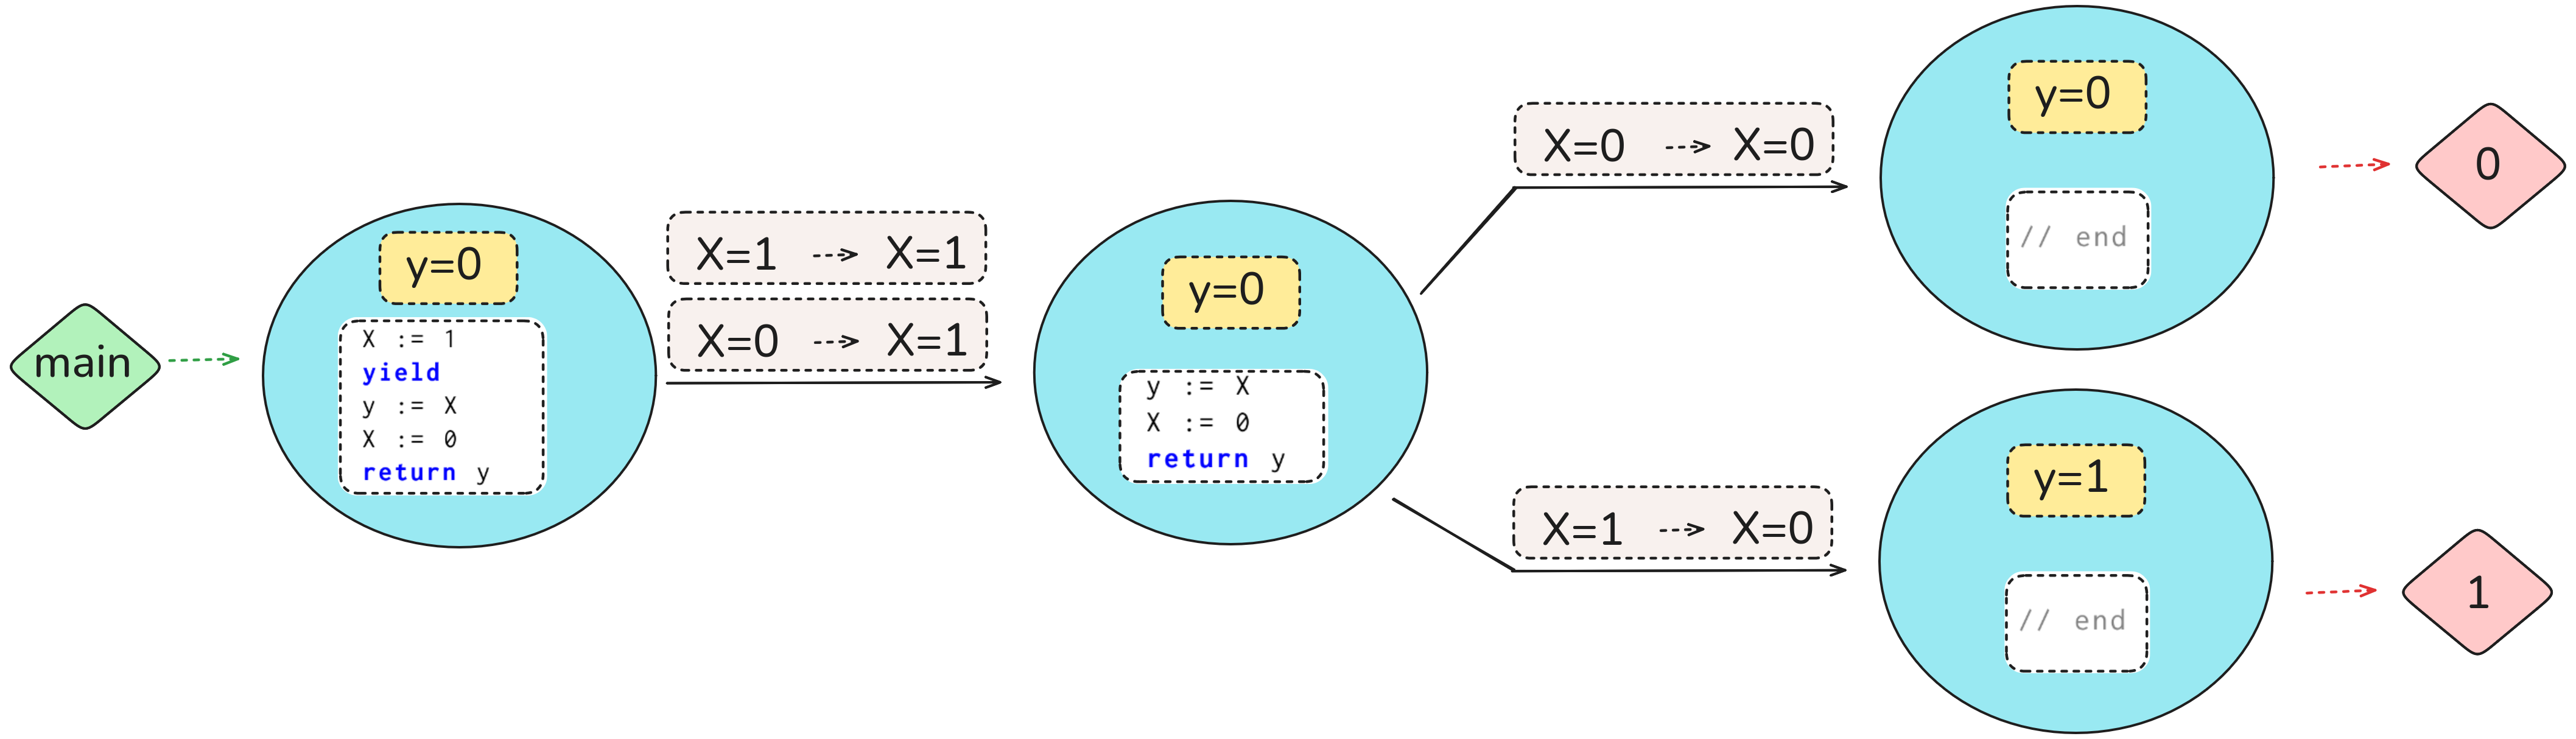
\includegraphics[width=\textwidth]{plots/code_2_NS.png}\\[1ex]

	\begin{tikzpicture}[
		node distance=1.5cm and 2.5cm,
		>=stealth,
		thick,
		every node/.style={font=\small}
	]
	  % [main request] -> [y=0][full program below that] ---[X=1 -> X=1][X=0 -> X=1 below that]--->[y=0][rest of program below that]
	  %   (first outgoing edge of last node on previous line)
      %   --[X=0 -> X=0]-->[y=0][empty program below that] ---> [0 response]
	  %   (second outgoing edge)
	  %   --[X=1 -> X=0]-->[y=1][empty program below that] ---> [1 response]
	  
	  % Main request node
	  \node[
		draw=black,
		line width=0.8pt,
		fill=ForestGreen!20,
		text=black,
		diamond,
		aspect=2,
		inner sep=2pt,
		scale=0.7
	  ] (main) {\texttt{main}};
	  
	  % First state node with full program
	  \node[right=0.7cm of main, align=center] (state1) {
		\begin{tikzpicture}[baseline=(ybox.base)]
			\node[
			draw=black,
			line width=0.8pt,
			fill=brightyellow,
			text=black,
			rectangle,
			rounded corners=1pt,
			inner sep=2pt
			] (ybox) {\texttt{y=0}};
		\end{tikzpicture}\\[-2.5pt]
		\begin{minipage}{2cm}
			\begin{lstlisting}[language=CustomPseudoCode,numbers=none,basicstyle=\tiny\ttfamily]
X := 1
yield
y := X
X := 0
return y
			\end{lstlisting}
		\end{minipage}
	  };
	  
	  % Second state node with rest of program
	  \node[right=of state1, align=center] (state2) {
		\begin{tikzpicture}[baseline=(ybox.base)]
			\node[
			draw=black,
			line width=0.8pt,
			fill=brightyellow,
			text=black,
			rectangle,
			rounded corners=1pt,
			inner sep=2pt
			] (ybox) {\texttt{y=0}};
		\end{tikzpicture}\\[-2.5pt]
		\begin{minipage}{1.5cm}
			\begin{lstlisting}[language=CustomPseudoCode,numbers=none,basicstyle=\tiny\ttfamily]
y := X
X := 0
return y
			\end{lstlisting}
		\end{minipage}
	  };
	  
	  % Final state y=0 with empty program
	  \node[above right=-0.5cm and 2.2cm of state2, align=center] (state3) {
		\begin{tikzpicture}[baseline=(ybox.base)]
			\node[
			draw=black,
			line width=0.8pt,
			fill=brightyellow,
			text=black,
			rectangle,
			rounded corners=1pt,
			inner sep=2pt
			] (ybox) {\texttt{y=0}};
		\end{tikzpicture}\\[-2.5pt]
		\begin{minipage}{0.8cm}
			\begin{lstlisting}[language=CustomPseudoCode,numbers=none,basicstyle=\tiny\ttfamily]
// end
			\end{lstlisting}
		\end{minipage}
	  };
	  
	  % Final state y=1 with empty program
	  \node[below right=-0.2cm and 2.2cm of state2, align=center] (state4) {
		\begin{tikzpicture}[baseline=(ybox.base)]
			\node[
			draw=black,
			line width=0.8pt,
			fill=brightyellow,
			text=black,
			rectangle,
			rounded corners=1pt,
			inner sep=2pt
			] (ybox) {\texttt{y=1}};
		\end{tikzpicture}\\[-2.5pt]
		\begin{minipage}{0.8cm}
			\begin{lstlisting}[language=CustomPseudoCode,numbers=none,basicstyle=\tiny\ttfamily]
// end
			\end{lstlisting}
		\end{minipage}
	  };
	  
	  % Response 0
	  \node[
		right=0.6cm of state3,
		draw=black,
		line width=0.8pt,
		fill=RedViolet!20,
		text=black,
		diamond,
		aspect=2,
		inner sep=2pt,
		scale=0.7,
		font=\Large
	  ] (resp0) {\texttt{0}};
	  
	  % Response 1
	  \node[
		right=0.6cm of state4,
		draw=black,
		line width=0.8pt,
		fill=RedViolet!20,
		text=black,
		diamond,
		aspect=2,
		inner sep=2pt,
		scale=0.7,
		font=\Large
	  ] (resp1) {\texttt{1}};
	  
	  % Arrows
	  \draw[->] (main) -- (state1);
	  
	  % Transition labels for state1 to state2
	  \draw[->] (state1) -- node[above] {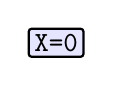
\begin{tikzpicture}[baseline=(a.base)]\node[draw=black,line width=0.8pt,fill=blue!10,rectangle,rounded corners=1pt,inner sep=2pt] (a) {\texttt{X=0}};\end{tikzpicture} $\to$ 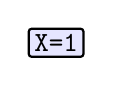
\begin{tikzpicture}[baseline=(b.base)]\node[draw=black,line width=0.8pt,fill=blue!10,rectangle,rounded corners=1pt,inner sep=2pt] (b) {\texttt{X=1}};\end{tikzpicture}} node[below] {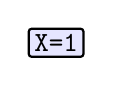
\begin{tikzpicture}[baseline=(c.base)]\node[draw=black,line width=0.8pt,fill=blue!10,rectangle,rounded corners=1pt,inner sep=2pt] (c) {\texttt{X=1}};\end{tikzpicture} $\to$ 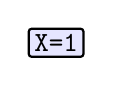
\begin{tikzpicture}[baseline=(d.base)]\node[draw=black,line width=0.8pt,fill=blue!10,rectangle,rounded corners=1pt,inner sep=2pt] (d) {\texttt{X=1}};\end{tikzpicture}} (state2);
	  
	  % From state2 to final states
	  \draw[->] ([yshift=4pt]state2.east) to[out=50,in=180] node[above, sloped] {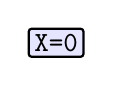
\begin{tikzpicture}[baseline=(a.base)]\node[draw=black,line width=0.8pt,fill=blue!10,rectangle,rounded corners=1pt,inner sep=2pt] (a) {\texttt{X=0}};\end{tikzpicture} $\to$ 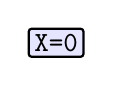
\begin{tikzpicture}[baseline=(b.base)]\node[draw=black,line width=0.8pt,fill=blue!10,rectangle,rounded corners=1pt,inner sep=2pt] (b) {\texttt{X=0}};\end{tikzpicture}} (state3.west);
	  \draw[->] ([yshift=-16pt]state2.east) to[out=-50,in=180] node[below, sloped] {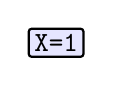
\begin{tikzpicture}[baseline=(a.base)]\node[draw=black,line width=0.8pt,fill=blue!10,rectangle,rounded corners=1pt,inner sep=2pt] (a) {\texttt{X=1}};\end{tikzpicture} $\to$ 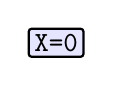
\begin{tikzpicture}[baseline=(b.base)]\node[draw=black,line width=0.8pt,fill=blue!10,rectangle,rounded corners=1pt,inner sep=2pt] (b) {\texttt{X=0}};\end{tikzpicture}} (state4.west);
	  
	  % To responses
	  \draw[->] (state3) -- (resp0);
	  \draw[->] (state4) -- (resp1);
	  
	\end{tikzpicture}
\caption{Network system for Listing~\ref{lst:MotivatingExample2NonSer}.
Local states show local assignments (yellow) and remaining code; edges show global-state transitions (blue). Requests/responses are green/red diamonds. Shapes (diamonds vs. rectangles) aid grayscale printing.}
%	\caption{The Network system for Listing~\ref{lst:MotivatingExample2NonSer}. 
%		Local states include (\textcolor{orange}{yellow}) local variable assignments and the remaining program; edges are labeled with (\textcolor{blue}{blue}) global state transitions. 
%		Requests and responses are shown as \textcolor{ForestGreen}{green} and \textcolor{red}{red} diamonds, respectively. 
%		From left to right: a \texttt{main} request spawns a thread with \texttt{[y=0]} and the full program; after yielding, $\delta$ advances to a step with global \texttt{[X=1]} and local \texttt{[y=0]} plus the remaining three expressions,; \texttt{y} is updated based on the global value, and \texttt{y}'s final assignment is the returned response.}

%		Network system for the program in Listing~\ref{lst:MotivatingExample2NonSer}. Local states consist of local variable assignments and a remaining program. Edges in the NS are labeled with their corresponding global state transition(s). Requests and responses are diamonds. 
	%
%	From left to right: a \texttt{main} request spawns a thread with \texttt{[y=0]} and the full program; after yielding, the $\delta$ transitions to a step in which  (globally) \texttt{[X=1]} and (locally) \texttt{[y=0]} with the remaining three expressions, etc.
	%	
%	For the explicit schemes of \(\delta\), \(req\), and \(resp\) see Appendix~\ref{appendix:delta-req-resp-examples}.
%}
\label{fig:code2ExampleNS}
\end{figure}
